% !TeX encoding = UTF-8
% !TeX spellcheck = en_US
% !TeX root = ../hdr_dfolio.tex

\Chapitre{Context of Activities}

This chapter introduces the various activities that I have conducted since I started as Associate Professor in 2008. It first starts with an overall overview of my career, that sets the context in which  my works was carried out.
As in any faculty position, my work encompasses several activities mainly related to teaching and research.
The organization of these tasks are then presented in \autoref{sec:activities}.
This integrates the articulations of the teaching, research, supervisions and collaboratives works in a general framework synergy.
This chapter largely refers to the appendices\;\RefCV and \RefMyRef that include a long version of my resume, and the list of my publications respectively.

\vskip1em plus 1fill

\section{Career overview}\label{sec:career}

\subsection{Doctorate degree and post-doctorate}\label{sec:career:PhD}

I defended my PhD in Robotics in 2007 within the  Robotics, Action, and Perception (RAP) group of the Laboratory for Analysis and Architecture of Systems (LAAS\footnote{LAAS: \url{http://www.laas.fr}}), CNRS\footnote{French National Center for Scientific Research, \url{http://www.cnrs.fr}}, under the supervision of Viviane Cadenat, Associate Professor at Paul Sabatier University in Toulouse. 
My PhD thesis dealt with the design of multi-sensor based control strategies allowing a mobile robot to perform vision-based tasks amidst possibly occluding obstacles.
We have first proposed techniques able to fulfill simultaneously the two previously
mentioned objectives. However, avoiding both collisions and occlusions often over-strained the
robotic navigation task, reducing the range of realizable missions. This is the reason why we have developed a second approach which lets the visual features loss occurs if it is necessary for the task realization. Using the link between vision and motion, we have proposed different methods (analytical and numerical) to compute the visual signal as soon it becomes unavailable. We have then applied them to perform vision-based tasks in cluttered environments, before highlighting their interest to deal with a camera failure during the mission.

Between 2007 and 2008, I joined the Lagadic team at \French{Inria Rennes-Bretagne Atlantique} as a postdoctoral fellow on sensory control for unmanned aerial vehicles. 
My postdoctoral fellow  has been supported by Sensory Control for Unmanned Aerial Vehicles (SCUAV) \ANR project.
The main objective was to improve multi-sensor-based servoing tasks for  unmanned aerial vehicles.
The idea was to design robust control law that combine different sensory data directly at the control level.
Especially, I have contributed to the design of a new on-line sensor self-calibration based on the sensor/robot interaction links \citep{2010_icra_kermorgant}%\CICL{2010_icra_kermorgant}.

\pagebreak[3]
\subsection{Tenured as Associate Professor}\label{sec:career:tenure}

In 2008, I was recruited as Associate Professor of the 61\up{st} CNU section at \ENSI Bourges, which is now  the \INSA \CVL\footnote{INSA \CVL (INSA CVL) was created in 2014 by the merge of \French{\'Ecole Nationale d'Ingénieurs du Val de Loire} (ENIVL) of Blois and ENSI of Bourges. In 2015, the \French{\'Ecole Nationale Supérieure de la Nature et du Paysage} (ENSNP) of Blois is integrated to INSA \CVL. \url{http://www.insa-centrevaldeloire.fr}}. 
\autoref{fig:timeline} shows the relevant events related with my activities.
Since then, I have been regularly involved in the life of the institute. 
In particular, I contribute at a local level to the scientific animations (eg., organization of laboratory visits), transfer and training-research links. 
Thus, I regularly attend the international relations division by accompanying the different delegations of schools and  universities partners during their visits to \INSA \CVL.
In March 2017, the direction of the \INSA \CVL  given to me the mission of referent \enquote{racism and antisemitism}.

As senior lecturer, I am mainly involved in the development of electronics and electrical sciences teaching activities of the institute.
In particular, I have contributed to develop all of the teaching materials for the electronics and electrical sciences  courses and tutorials.
Since September 2014, I am in charge of the Nuclear Energy options of the 5\up{th} year (engineer's degree) of the Industrial Risk Control (MRI\footnote{\French{Ma\^itrise des Risques Industriels (MRI)}}) department.

\medskip

\begin{figure}[tbh]
  \centering
  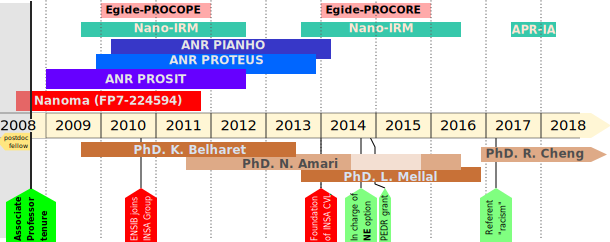
\includegraphics[width=1\linewidth-1pt]{fig/chapI/dfolio_timeline} %
  \caption[Progress of main events and activities.]{Progress of main events and activities (\eg projects and supervisions) related since my tenure.}
  \label{fig:timeline}
\end{figure}
%
\begin{figure}[tbh]
  \centering
  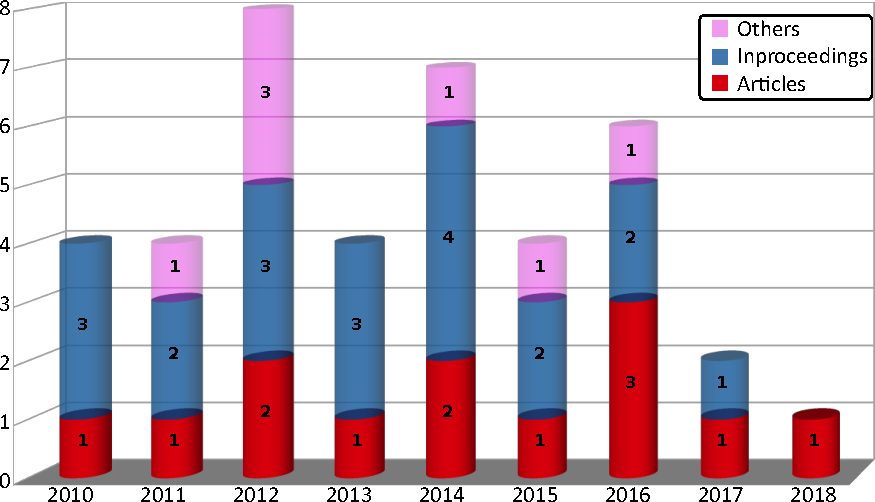
\includegraphics[scale=1]{fig/chapI/dfolio_publis} %width=1\linewidth-1ex
  \caption[Personal references timeline.]{Personal references timeline evolution.}
  \label{fig:publis}
\end{figure}

Furthermore, I perform my research activities with the \PRISMEfoot  Laboratory in the Robotics axis of the IRAuS pole.
My research interests mainly deal with modeling and control for nano and micro-robotics in a biomedical context.
In a first time, my research activities have been mainly related with the European project \NANOMAfoot.
This project consisted to design microrobotic system for targeted drug delivery through the cardiovascular system.
Parallelly, I have also contributed to the development of micromanipulation activities of the laboratory.
Firstly, the micromanipulation has been devoted for intra-cytoplasmic applications \cite{2011_icra_kim,2012_tase_kim}.
Next, this research activities evolved to object micromanipulation to be placed in the focus of a light beam within the \ANRfoot project \PIANHOfoot.
The different projects in which I have been involved are reported in the \autoref{fig:timeline}, and detailed in appendix\;\RefAnnexeCV.XX.
I have co-supervised 4 PhD thesis (with one still on going) also shown in the \autoref{fig:timeline}, and detailed in appendix\;\RefAnnexeCV.YY.
Since 2018, I have contributed to 40 publications, including 12 articles and 20 proceedings.
\autoref{fig:publis} illustrate the timeline progress of my publishing activities and the detailed list of my publications are given in appendix\;\RefAnnexeRef. 



\section{Activities Organization}\label{sec:activities}

\subsection{Teaching activities}\label{sec:teaching}
\subsection{Research Field}\label{sec:research}


\section{Manuscript Overview}\label{sec:org}
